\section{\bt{Design of \system}{\system\ 的设计}}
\label{sec:model}
\label{sec:design}
\bi{Using analytical metrics as our primary case, we present the shared representation and three-layer generalization boundary (Section~\ref{sec:shared-object}), verification-guided extraction for C1 (Section~\ref{sec:publication}), condition-grounded lookup and audit control for C2 (Section~\ref{sec:lookup}), and for C3 the validity conditions (Section~\ref{sec:sufficiency}) and their two-stage maintenance and snapshot-bound execution (Section~\ref{sec:maintenance}). Sections~\ref{sec:optimization} and~\ref{sec:features} extend these mechanisms to query optimization and predictive features.}
{本节以分析型指标为主线，依次介绍共享表示与三层泛化边界（第~\ref{sec:shared-object} 节）、针对 C1 的验证引导提取（第~\ref{sec:publication} 节）、针对 C2 的有据查找与审计控制（第~\ref{sec:lookup} 节），以及针对 C3 的有效性条件（第~\ref{sec:sufficiency} 节）和两级增量维护与快照绑定执行（第~\ref{sec:maintenance} 节）。第~\ref{sec:optimization} 与~\ref{sec:features} 节将其扩展至查询优化与预测特征。}

\subsection{\bt{Shared Representation and Generalization Boundary}{共享表示与泛化边界}}
\label{sec:shared-object}
\bi{Each metric definition revision is stored as a tuple}
{每个指标定义版本表示为如下元组：}
\begin{equation}
\label{eq:metric-revision}
m^r=(B,I,C,E,r),
\end{equation}
\bi{where $B$ specifies the business meaning, $I$ encodes the structured relational implementation, $C=C(m^r)$ is the set of executable data conditions derived from $I$ and from the session's exploration probes (Section~\ref{sec:sufficiency}), $E$ records the learning provenance (source request, verified calculation trace, dependency version vector, and publication checks), and $r$ is the revision number. Subscripts ($m_i^r$) distinguish metrics, whereas $m^r\to m^{r+1}$ updates one metric's revision. A feature revision $f^r$ shares this tuple, extending $I$ with entity mappings, look-back windows, and fill values (Section~\ref{sec:features}).}
{其中，$B$ 描述业务含义，$I$ 规定结构化关系实现，$C=C(m^r)$ 为从 $I$ 与会话探针推导出的可执行数据条件集（第~\ref{sec:sufficiency} 节），$E$ 记录学习溯源（源请求、核验计算链、依赖表版本向量及发布检查结果），$r$ 为版本号。下标（$m_i^r$）区分不同指标，而 $m^r\to m^{r+1}$ 表示同一指标的版本演进。特征版本 $f^r$ 采用同一元组表示，在 $I$ 中扩展实体映射、回看窗口与默认填充值（第~\ref{sec:features} 节）。}

\bi{\emph{Three-layer generalization boundary.} To prevent under- or over-generalization across sessions (C1) and provide an exact coverage criterion for lookup (C2), \system{} partitions a reusable computation into three layers (Figure~\ref{fig:extraction}, top right):
(1)~\emph{Fixed core semantics ($I$)}: fact table $F$, aggregate operator $\mathrm{AGG}$ over measure expression $e$, business grain key $K$, verified many-to-one join tree $\mathcal J$ rooted at $F$, domain filter $\varphi$ (e.g., \code{i\_category = 'Electronics'}), and time attribution $\tau$ (an event-time column on $F$ or a fact-to-date-dimension join). Changing any element of $(F, \mathrm{AGG}_{e}, K, \mathcal J, \varphi, \tau)$ alters the business metric and requires a new definition.
(2)~\emph{Admissible parameters ($p$)}: request bindings that select a reporting period $p$ for metrics or an entity and cutoff $(u_i, t_i)$ for features without modifying $I$.
(3)~\emph{Admissible post-aggregation derivations ($d$)}: deterministic operations composed over the base aggregate, namely slicing or ranking by an attribute reachable from $F$ through $\mathcal J$, or computing differences across two parameter bindings $(p_1, p_2)$.}
{\emph{三层泛化边界。}为避免跨会话泛化不足或过度泛化（C1），并为查找提供准确的覆盖判据（C2），\system{} 将可复用计算显式划分为三层（图~\ref{fig:extraction} 右上）：(1)~\emph{固定核心语义（$I$）}：事实表 $F$、度量表达式 $e$ 上的聚合算子 $\mathrm{AGG}$、业务粒度键 $K$、以 $F$ 为根的已验证多对一连接树 $\mathcal J$、业务域过滤 $\varphi$（如 \code{i\_category = 'Electronics'}）以及时间归属 $\tau$（$F$ 上的事件时间列或事实表到日期维表的连接）。改变 $(F, \mathrm{AGG}_{e}, K, \mathcal J, \varphi, \tau)$ 的任一要素均构成不同指标，须建立新定义。(2)~\emph{允许变化的参数（$p$）}：在不改变 $I$ 的前提下由请求提供的绑定值，如指标报告期间 $p$ 或特征实体与截点 $(u_i, t_i)$。(3)~\emph{允许的聚合后派生操作（$d$）}：在基础聚合之上复合的确定性操作，包括按从 $F$ 经 $\mathcal J$ 可达的属性分组切片或排序，以及计算两个参数期间 $(p_1, p_2)$ 的差值。}

\bi{Let $J_I(D_s)$ denote the relation obtained by applying $\mathcal J$, $\tau$, and $\varphi$ to database snapshot $D_s$. Given parameter $p$ and optional derivation $d$, compilation emits a read-only query $q=\operatorname{Compile}(I,p,d)$:}
{设 $J_I(D_s)$ 为在快照 $D_s$ 上应用连接树 $\mathcal J$、时间归属 $\tau$ 与过滤 $\varphi$ 后得到的关系。给定参数 $p$ 与可选派生操作 $d$，编译生成只读查询 $q=\operatorname{Compile}(I,p,d)$：}
\begin{equation}
\label{eq:compiled-metric}
q_0(D_s, p)=\mathrm{AGG}_{e}\bigl(\sigma_{\tau\in p}(J_I(D_s))\bigr), \;\; q(D_s)=d\bigl(q_0(D_s, p)\bigr),
\end{equation}
\bi{where $d$ is the identity map for scalar period queries. Because $I$ and its conditions $C(m^r)$ are invariant to $p$ and $d$, Agents~1, 2, and $N$ in Figure~\ref{fig:architecture} reuse one verified implementation across distinct periods, rankings, and comparisons.}
{其中标量期间查询的 $d$ 为恒等映射。由于核心实现 $I$ 及其数据条件 $C(m^r)$ 不随 $p$ 和 $d$ 改变，图~\ref{fig:architecture} 中的智能体 1、2 与 $N$ 可跨不同期间、排名与同比差值安全复用同一核验定义。}

\subsection{\bt{Verification-Guided Extraction and Publication}{验证引导的定义提取与受检发布}}
\label{sec:publication}
\begin{figure}[t]
\centering
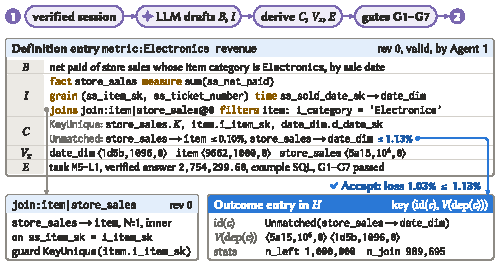
\includegraphics[width=\columnwidth]{figures/extraction}%
\caption{\bt{Definition extraction, generalization boundary, condition derivation, and publication gates (G1--G7) in steps 1--2.}{步骤 1--2 中的定义提取、三层泛化边界、条件推导与发布准入（G1--G7）。}}
\label{fig:extraction}
\Description{Definition extraction, three-layer generalization boundary, structural and probe-lifted conditions, and publication gates G1 to G7.}
\end{figure}

\bi{To address C1, \emph{Publish} extracts a candidate definition from a verified session and enforces seven admission gates G1--G7 (Figure~\ref{fig:extraction}). Given the session's question, verified answer, and SQL/probe trace, an LLM extractor separates fixed semantics $I$ from the session's parameter $p_0$ and derivation $d_0$, while the server derives structural and probe-lifted conditions $C(m^r)$ (Section~\ref{sec:sufficiency}). Admission checks three properties:
(1)~\emph{Source support} verifies that $B$ cites a concrete business basis (G1) and that the arithmetic trace matches the verified answer (G2).
(2)~\emph{Structural admissibility} verifies that all tables, columns, expressions, many-to-one joins $\mathcal J$, and domain filters $\varphi$ exist with query-specific literals lifted into $p_0$ (G3), checks key uniqueness at the declared fact grain $K$ (G4), and validates that the example SQL is a single read-only query (G5).
(3)~\emph{Answer reproduction} guards against lossy extraction: as shown at the bottom of Figure~\ref{fig:extraction}, raw session SQL can reproduce the answer (G6) even when the extracted $I$ accidentally drops a mandatory filter such as $\varphi$. \system{} therefore compiles $\operatorname{Compile}(I,p_0,d_0)$ solely from the extracted structure $I$ and requires its output on the unchanged learning tables to match the verified session answer at task precision (G7) before publishing $m^{r_0}$.}
{针对 C1，\emph{发布}模块从核验会话中提取候选定义，并执行七项准入检查 G1--G7（图~\ref{fig:extraction}）。给定会话问题、核验答案与 SQL／探针轨迹，提取器将固定核心语义 $I$ 与会话参数 $p_0$、派生操作 $d_0$ 分离，服务端推导结构条件与探针条件 $C(m^r)$（第~\ref{sec:sufficiency} 节）。准入检验三方面性质：(1)~\emph{来源支持}核实业务含义 $B$ 具明确依据（G1）且算术链与核验答案一致（G2）；(2)~\emph{结构合法性}验证 $I$ 中表、列、表达式、多对一连接 $\mathcal J$ 与过滤 $\varphi$ 合法且查询字面量已提为参数 $p_0$（G3），检验事实表在粒度 $K$ 上的键唯一性（G4），并确认示例 SQL 为单条只读查询（G5）；(3)~\emph{答案复现}防止有损提取：如图~\ref{fig:extraction} 底部所示，即便提取的 $I$ 遗漏了必需过滤 $\varphi$，原始会话 SQL 仍可复现答案（G6）。因此 \system{} 仅由提取结构 $I$ 编译执行 $\operatorname{Compile}(I,p_0,d_0)$，要求其在未变学习表上精确复现核验答案（G7）后方才发布 $m^{r_0}$。}

\subsection{\bt{Condition-Grounded Lookup and Audit Control}{基于条件的有据查找与审计控制}}
\label{sec:lookup}
\begin{figure}[t]
\centering
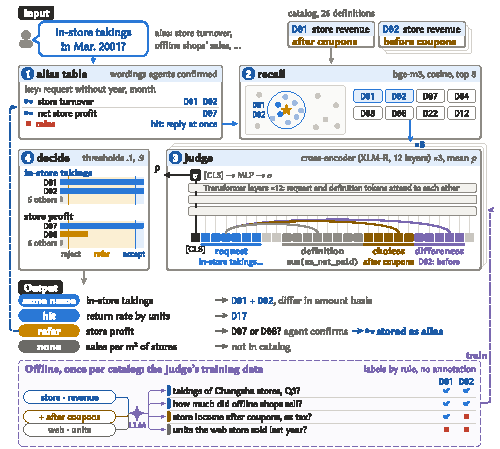
\includegraphics[width=\columnwidth]{figures/lookup}%
\caption{\bt{Accurate lookup via monthly row-contribution fingerprints in evidence graph $G$ (a) and online constraint-explaining admission (b).}{基于按月行级贡献指纹与证据关联图 $G$（a）及在线约束解释准入（b）的准确查找。}}
\label{fig:lookup}
\Description{Monthly row-contribution fingerprint and evidence graph G with definitions X, Y, Z on a 3-row sales table, and online constraint-explaining request admission.}
\end{figure}

\begin{algorithm}[t]
\caption{\bt{Constraint-explaining lookup and post-hoc graph update}{约束解释查找与事后关联图更新}}
\label{alg:lookup}
\small
\begin{algorithmic}[1]
\Require Request $\rho$; evidence graph $G$; snapshot $s$; risk bound $\alpha$
\Ensure Answer, clarification, partial hit, or exploration result
\Function{Lookup}{$\rho, G, s, \alpha$}
  \State $A(\rho) \gets \operatorname{Parse}(\rho)$; $\; K \gets \operatorname{Candidates}(A(\rho), G)$
  \State $S \gets \{m \in K \mid \operatorname{Res}(\rho,m)=\varnothing \wedge \neg\operatorname{Excl}(\rho,m) \wedge P_{\mathrm{route}}(D_s)\}$
  \IfThen{$S = \varnothing$}{\Return $\text{PartialHit}(m,\operatorname{Res})$ if matched, else $\text{Miss}$}
  \IfThen{$\lvert S\rvert = 1 \wedge \rho \in \Phi(S)$}{\Return $\operatorname{CheckAndRun}(S, \rho, s)$}
  \State $Y \gets \{\operatorname{CheckAndRun}(m,\rho,s) \mid m \in S\}$ \Comment{indifference test}
  \IfThen{$\lvert Y\rvert > 1$}{\Return $\text{Clarify}(\delta, Y)$} \Comment{else outputs agree on $D_s$}
  \State $g \gets \operatorname{Stratum}(\rho, S)$ \Comment{tentative match: check audit bound}
  \IfThen{$U_g(t) \le \alpha \wedge \neg\operatorname{ResidualAudit}()$}{\Return value in $Y$}
  \State $u \gets \operatorname{Explore}(\rho, s)$; $\; \ell \gets \Call{RecordAndLabel}{u, \rho, S, s}$
  \State Update $U_g(t+1)$ with $z = \mathbb{1}[\ell \neq \text{equiv}]$; \Return output of $u$
\EndFunction
\Function{RecordAndLabel}{$u, \rho, S, s$}
  \For{each definition $m$ on $u$'s fact table}
    \IfThen{$I_u \equiv_P I_m$ on $D_s$}{Add $(u, m, P)$ to $G$; add $\rho$ to $\Phi(m)$}
    \IfThen{$0 < \lvert\delta(u,m)\rvert \le 2$}{Add contrast $(u, m, \delta)$ and modifier}
  \EndFor
  \State \Return $\text{equiv}$ if $\exists m\in S: I_u \equiv_P I_m$, $\text{distinct}$ if $\not\equiv$, else $\text{unprovable}$
\EndFunction
\end{algorithmic}
\end{algorithm}

\bi{To address C2 without generating full SQL for an incoming request $\rho$, \system{} separates offline relational verification from online constraint-explaining admission (Figure~\ref{fig:lookup} and Algorithm~\ref{alg:lookup}), distinguishing three levels of guarantees:
(1)~\emph{Certified definition equivalence ($u \equiv_P m$)}, proving that normalized implementations $I_u$ and $I_m$ compute identical relations for all $p$ whenever database premises $P$ hold;
(2)~\emph{Grounded request templates ($\Phi(m)$) and contrastive modifiers ($\delta(u,m)$)}, binding verified natural-language templates and modifier phrases to specific parameter slots, derivations, and differing fields of $I$; and
(3)~\emph{Snapshot value agreement}, running surviving candidates on the current snapshot $D_s$ to skip user clarification when they return identical outputs under the premise that the intended computation lies within the candidate set.}
{为在不预先为新请求 $\rho$ 生成完整 SQL 的情况下解决 C2，\system{} 将事后关系验证与在线约束解释准入相分离（图~\ref{fig:lookup} 与算法~\ref{alg:lookup}），严格区分三层保证：(1)~\emph{认证定义等价（$u \equiv_P m$）}，证明两个规范化实现 $I_u$ 与 $I_m$ 在数据库前提 $P$ 成立时对任意参数 $p$ 结果恒等；(2)~\emph{接地请求模板（$\Phi(m)$）与差异修饰词（$\delta(u,m)$）}，将经核验的自然语言模板和修饰词绑定到特定的参数槽位、派生操作及 $I$ 的差异字段；(3)~\emph{快照同值检验}，在目标意图属于幸存候选集的前提下，通过在当前快照 $D_s$ 上执行候选定义，当输出同值时免去向用户追问。}

\bi{\emph{1. Post-hoc evidence graph ($G$).} Whenever a verified computation $u$ is obtained---at publication, after a miss exploration, or during an audit---\system{} normalizes $I_u$ (ordering joins and filter conjuncts, qualifying columns, and canonicalizing $e$) and compares it against every definition $m$ on the same fact table (\textsc{RecordAndLabel} in Algorithm~\ref{alg:lookup}). If normalized forms differ, \system{} tests three conditional rewrite rules, each requiring an explicit database condition $P$:
(R1)~drop an unreferenced, filter-free left join if its right table is unique on the join key;
(R2)~drop such an inner join if, in addition, no left row is unmatched; and
(R3)~replace a date-dimension period join with a range predicate on the fact's date key if date keys are contiguous by month.
When $I_u$ and $I_m$ converge under rules whose premises $P$ hold on $D_s$, \system{} records a \emph{certified equivalence edge} $(u, m, P)$. Otherwise, if $I_u$ and $I_m$ differ in at most two fields $\delta(u,m) \subseteq \{e, K, \varphi, \mathcal J, \tau\}$, \system{} adds a \emph{contrast edge} $(u, m, \delta)$. Pairs that R1--R3 cannot relate receive no equivalence edge even if their outputs coincide on $D_s$.}
{\emph{1. 事后证据关联图（$G$）。}每当在发布、未命中探索或审计中获得经核验计算 $u$ 时，\system{} 将 $I_u$ 规范化（连接与过滤排序、列名限定、表达式规范化），并与同一事实表上的定义 $m$ 比对（算法~\ref{alg:lookup} 中的 \textsc{RecordAndLabel}）。若规范形式不同，系统测试三条以显式数据条件 $P$ 为前提的改写规则：（R1）若右表在连接键上唯一，移除未提供被引用列且无过滤的左连接；（R2）若此外无未匹配左侧行，移除此类内连接；（R3）若日期键按月连续，将日期维表连接替换为事实表日期键上的范围谓词。当 $I_u$ 与 $I_m$ 在当前状态 $D_s$ 上前提 $P$ 成立的规则下收敛一致时，记录\emph{认证等价边} $(u, m, P)$；否则若二者仅在至多两个字段 $\delta(u,m) \subseteq \{e, K, \varphi, \mathcal J, \tau\}$ 上不同，则添加\emph{差异边} $(u, m, \delta)$。无法由 R1--R3 证明等价的定义对即便在当前数据上输出相同也不建立等价边。}

\begin{proposition}[\bt{Certified conditional equivalence}{认证条件等价}]
\label{prop:rewrite}
\bi{Let the date dimension's key be unique on database state $D_s$. (a) If date-key contiguity holds on $D_s$ (each month's keys form a contiguous integer interval immediately following the prior month's maximum key), definitions related by R3 agree for every consecutive-month period $p$. (b) If the right table of a removed left join is unique on its join key on $D_s$, definitions related by R1 agree for all $p$; if furthermore no left row is unmatched, definitions related by R2 agree for all $p$.}
{设日期维表主键在状态 $D_s$ 上唯一。（a）若日期键连续性在 $D_s$ 上成立（每月日期键构成紧接上月最大键的连续整数区间），则由 R3 关联的定义对任意连续月份期间 $p$ 输出一致。（b）若被移除左连接的右表在 $D_s$ 上满足连接键唯一，则由 R1 关联的定义对任意 $p$ 输出一致；若此外无未匹配左侧行，由 R2 关联的定义亦对任意 $p$ 输出一致。}
\end{proposition}
\begin{proof}[\bt{Proof sketch}{证明概要}]
\bi{(a) Contiguity maps any consecutive-month period to a closed integer interval of date keys, so a fact row satisfies the key-range predicate iff it joins with a date row in $p$. (b) A many-to-one left join projecting no column preserves every left row with multiplicity one; zero unmatched left rows makes the inner join identical.\qedhere}
{（a）连续性将任意连续月份期间映射为日期键的闭整数区间，事实行满足范围谓词当且仅当其连接到 $p$ 内的日期行。（b）不投影列的多对一左连接以重数 1 保留每条左侧行；无未匹配左侧行时内连接与之完全等价。\qedhere}
\end{proof}

\bi{Because $I$ fixes the grain $K$, time $\tau$, and measure $e$ with many-to-one joins, each definition also admits a \emph{monthly row-contribution fingerprint} $\mathrm{fp}(m, ym) = \sum_{r}\operatorname{hash}(K(r), ym(r), e(r))$ grouped by month (Figure~\ref{fig:lookup}a): additive hashing is order-independent and updates incrementally on append batches $\Delta T$ by summing new row hashes without rescanning the fact table. In Figure~\ref{fig:lookup}a, definitions \code{X} (no dimension join) and \code{Z} (\code{JOIN item}, zero rows lost under R2) produce identical fingerprints in both \code{2002-09} and \code{2002-10} ($\mathrm{X} \equiv_P \mathrm{Z}$), whereas \code{Y} (\code{JOIN store}) drops row \code{102B} (\code{store=NULL}) in \code{2002-09} ($\delta=\{\mathcal J_{\mathrm{store}}\}$) yet agrees with \code{X} in \code{2002-10}. Each verified pair $(u, \rho)$ populates a \emph{grounded request template} in $\Phi(m)$ for $u$ and any $m$ with $u \equiv_P m$ (storing the verification source, masked template, verified $(p, d)$ bindings, and routing premise $P_{\mathrm{route}}$), while contrast edges $(u, m, \delta)$ pair endpoint templates to isolate contrastive modifiers.}
{由于 $I$ 固定了粒度键 $K$、时间 $\tau$、度量 $e$ 及多对一连接，每个定义均可按月计算\emph{行级贡献指纹} $\mathrm{fp}(m, ym) = \sum_{r}\operatorname{hash}(K(r), ym(r), e(r))$（图~\ref{fig:lookup}a）：加法哈希与行序无关，且在追加批次 $\Delta T$ 时仅需对新增行算哈希累加而无需重扫全表。图~\ref{fig:lookup}a 中，定义 \code{X}（直接聚合销售表）与 \code{Z}（内连接商品表，在 R2 下零丢行）在 \code{2002-09} 与 \code{2002-10} 指纹完全相同（$\mathrm{X} \equiv_P \mathrm{Z}$）；而 \code{Y}（内连接门店表）因 \code{102B} 门店为空在 \code{2002-09} 少算一行（$\delta=\{\mathcal J_{\mathrm{store}}\}$），但在 \code{2002-10} 与 \code{X} 指纹一致。每次核验通过的 $(u, \rho)$ 还在 $\Phi(m)$ 中为 $u$ 及满足 $u \equiv_P m$ 的定义登记一条\emph{接地请求模板}（保存核验来源、掩码模板、$(p, d)$ 绑定与路由前提 $P_{\mathrm{route}}$），差异边 $(u, m, \delta)$ 则比对两端模板以锚定差异修饰词。}

\bi{\emph{2. Online constraint-explaining admission.} Because relational equivalence $I_u \equiv_P I_m$ cannot prevent a parser from dropping a natural-language qualifier in a new request $\rho$, one LLM call (without database probing) decomposes $\rho$ into constraints $A(\rho)$ (core computation phrase, attribute selections, time window, output shape) and retrieves candidates $K$ matching the phrase plus their $\delta$-neighbors (lines 2--3 of Algorithm~\ref{alg:lookup}). For $m\in K$, a constraint is \emph{explained} iff it binds to an admissible parameter $p$, an admissible derivation $d$, or an existing field of $I_m$; unexplained constraints form the residue $\operatorname{Res}(\rho, m)$, while modifiers matching a contrast edge $\delta(m, m')$ exclude $m$. Admission resolves four cases (Figure~\ref{fig:lookup}b):
\textbf{Case 1 (Grounded hit):} $\operatorname{Res}(\rho, m)=\varnothing$, $m$ is not excluded, the template is in $\Phi(m)$, and $P_{\mathrm{route}}(D_s)$ holds (line 5) $\to$ bind $(p,d)$ and run $m$.
\textbf{Case 2 (Contrast / Partial hit):} $\operatorname{Res}(\rho, m)\neq\varnothing$ (e.g., ``net of returns'' on \code{X}) $\to$ reject full reuse, pass $(m, \operatorname{Res})$ to the agent to complete only the missing filter/join, and record the verified result as a $\delta$-neighbor (line 4).
\textbf{Case 3 (Indifference Test):} When $\rho$ is silent on a contrasting field $\delta$ ($\lvert S\rvert > 1$, e.g., $S=\{\mathrm{X}, \mathrm{Y}\}$ in Figure~\ref{fig:lookup}b), \system{} checks whether the candidates in $S$ agree on the requested period and snapshot $D_s$ (lines 6--7): for \code{2002-10}, $\mathrm{fp}(\mathrm{X},10)=\mathrm{fp}(\mathrm{Y},10)$ so \system{} returns \code{20} immediately without asking; for \code{2002-09}, they differ and \system{} asks one clarification question on $\delta$. Period/snapshot agreement is strictly an online clarification optimization under the premise that the intended computation lies in $S$; it never adds an equivalence edge to $G$.}
{\emph{2. 在线约束解释准入与当期同值检验。}由于定义等价 $I_u \equiv_P I_m$ 无法防止自然语言解析在面对新请求 $\rho$ 时遗漏限定词，一次不访问数据库的轻量 LLM 调用将 $\rho$ 拆解为约束集 $A(\rho)$，并召回匹配候选及其 $\delta$ 邻居集 $K$（算法~\ref{alg:lookup} 第 2--3 行）。对 $m\in K$，约束被\emph{解释}当且仅当其绑定到参数 $p$、派生操作 $d$ 或 $I_m$ 已有字段；未解释约束构成残余 $\operatorname{Res}(\rho, m)$，匹配差异边的修饰词则排除 $m$。准入区分四种情形（图~\ref{fig:lookup}b）：\textbf{情形 1（接地命中）：}$\operatorname{Res}=\varnothing$、未被排除、模板在 $\Phi(m)$ 中且 $P_{\mathrm{route}}(D_s)$ 成立（第 5 行）$\to$ 直接绑定执行。\textbf{情形 2（部分命中）：}$\operatorname{Res}\neq\varnothing$（如残余``扣除退货''）$\to$ 拒绝完全复用，将 $(m, \operatorname{Res})$ 交给智能体仅补全缺失部分并记为 $\delta$ 邻居（第 4 行）。\textbf{情形 3（无差别检验）：}当请求未指明差异字段 $\delta$ 导致 $\lvert S\rvert > 1$（如图~\ref{fig:lookup}b 中 $S=\{\mathrm{X}, \mathrm{Y}\}$）时，系统检验候选在所问期间与快照 $D_s$ 上是否同值（第 6--7 行）：若问 \code{2002-10}，因 $\mathrm{fp}(\mathrm{X},10)=\mathrm{fp}(\mathrm{Y},10)$ 直接免追问返回 \code{20}；若问 \code{2002-09} 则因二者不同围绕 $\delta$ 发起单次澄清追问。当期同值仅是在``真实意图属于 $S$''前提下减少追问的在线优化，绝不向 $G$ 添加等价边。}

\bi{\emph{3. Three-way audit labels and false-hit bound (Case 4).} A surviving hit that rests on similarity rather than $\Phi(m)$ is \emph{tentative} and grouped into stratum $g$ (by match tier and contrast field types). When the confidence upper bound $U_g(t) > \alpha$ or a residual audit coin triggers (lines 8--11), the agent explores from scratch to obtain verified computation $u$, and \textsc{RecordAndLabel} assigns a three-way structural label $\ell$:
(i)~\emph{certified equivalent} ($\ell = \text{equiv}$), if $I_u \equiv_P I_m$ under active premises $P(D_s)$;
(ii)~\emph{confirmed distinct} ($\ell = \text{distinct}$), if $I_u$ and $I_m$ differ in core fields or outputs; or
(iii)~\emph{unprovable} ($\ell = \text{unprovable}$), if R1--R3 cannot prove equivalence despite matching outputs on $D_s$.
To bound risk conservatively without assuming rewrite completeness, $z_t = \mathbb{1}[\ell \neq \text{equiv}]$ counts both $\text{distinct}$ and $\text{unprovable}$ as non-certified failures when updating the $(1-\beta_g)$ confidence sequence $U_g(t)$ for stratum $g$'s non-equivalence rate $\mu_g$, while logging them separately for analysis.}
{\emph{3. 三值审计标签与误命中上界（情形 4）。}仅凭相似度而非接地模板 $\Phi(m)$ 的命中为\emph{待验证（tentative）}，按匹配层级与差异字段类型归入分层 $g$。当置信上界 $U_g(t) > \alpha$ 或触发小概率常驻抽检时（第 8--11 行），智能体独立探索得出核验计算 $u$，由 \textsc{RecordAndLabel} 给出三值结构标签 $\ell$：(i)~\emph{已证明等价}（$\ell = \text{equiv}$），即在活跃前提 $P(D_s)$ 下证明 $I_u \equiv_P I_m$；(ii)~\emph{已确认不同}（$\ell = \text{distinct}$），即核心字段或输出不同；(iii)~\emph{当前无法判定}（$\ell = \text{unprovable}$），即 $D_s$ 上输出相同但 R1--R3 无法证明等价。为在不假设改写完备的前提下保守控制风险，$z_t = \mathbb{1}[\ell \neq \text{equiv}]$ 将 $\text{distinct}$ 与 $\text{unprovable}$ 均计为失败以更新分层非等价率 $\mu_g$ 的 $(1-\beta_g)$ 置信序列上界 $U_g(t)$，同时分开记录二者。}

\begin{proposition}[\bt{Stratified false-hit bound}{分层误命中率上界}]
\label{prop:falsehit}
\label{prop:false-hit}
\bi{Within each stationary regime between resets of stratum $g$, suppose tentative hits in $g$ have i.i.d.\ indicators $z_t$ with mean $\mu_g \ge \Pr[\hat a_j \neq a^*_j \mid j\in g]$. With probability at least $1-\sum_g\beta_g$, every stratum ever served without audit satisfies $\mu_g \le \alpha$, bounding the expected false-hit rate across un-audited tentative hits by $\alpha$.}
{在分层 $g$ 两次重置间的平稳阶段内，设待验证命中的指示量 $z_t$ 独立同分布且均值 $\mu_g \ge \Pr[\hat a_j \neq a^*_j \mid j\in g]$。则以至少 $1-\sum_g\beta_g$ 的概率，所有获准免审计服务的分层均满足 $\mu_g \le \alpha$，免审计待验证命中的期望误命中率至多为 $\alpha$。}
\end{proposition}
\begin{proof}
\bi{Since $\ell=\text{equiv}$ implies $I_u \equiv_P I_m$ on $D_s$, every true mismatch has $z_t=1$, so $\Pr[\text{false hit}\mid g] \le \mu_g$. A time-uniform confidence sequence ensures $\forall t\ge 1: \mu_g \le U_g(t)$ with probability $\ge 1-\beta_g$; a union bound over strata and the gate $U_g(t)\le\alpha$ yield $\mu_g\le\alpha$.\qedhere}
{因 $\ell=\text{equiv}$ 蕴含 $D_s$ 上 $I_u \equiv_P I_m$，真实误匹配必有 $z_t=1$，故 $\Pr[\text{误命中}\mid g] \le \mu_g$。时间一致置信序列以至少 $1-\beta_g$ 概率对所有 $t$ 满足 $\mu_g \le U_g(t)$；取并集界并由门禁 $U_g(t)\le\alpha$ 即得 $\mu_g\le\alpha$。\qedhere}
\end{proof}
\bi{Proposition~\ref{prop:falsehit} enforces Constraint~\eqref{eq:correctness} up to finite-sample martingale concentration slack, and $U_g(t)$ is recalibrated whenever a new contrast edge splits $g$, a broken premise $P$ reverts routed templates to tentative, or the residual audit detects distribution drift.}
{命题~\ref{prop:falsehit} 在有限样本鞅集中范围内实现了约束~\eqref{eq:correctness}；当新增差异边细分 $g$、前提 $P$ 失效使路由模板退回待验证或常驻抽检发现漂移时，系统自动重校准 $U_g(t)$。}

\subsection{\bt{Validity Conditions and Guarantee Boundary}{有效性条件与保证边界}}
\label{sec:sufficiency}
\bi{To address C3, \system{} expresses the assumptions of both definitions $C(m^r)$ and C2 equivalence edges $P$ as checkable predicates over $\operatorname{dep}(c)$, each evaluated by a summary query $Q_c$ and acceptance rule $c(D_s)$. From $I$, \system\ derives five structural checks (markers 1--5 in Figure~\ref{fig:extraction}):
(1)~\emph{Filtered fact-grain uniqueness} $\operatorname{KeyUnique}(F,K,\varphi)$ across $\sigma_\varphi(F)$;
(2)~\emph{Join cardinality}, bounding each join edge in $\mathcal J$ to at most one right match per left row;
(3)~\emph{Inner-join} and (5)~\emph{Date-join completeness}, requiring the unmatched row fraction along each path to stay within publication baseline $b$ plus tolerance $\epsilon_{\mathrm{loss}}$ ($0$ for strict mode, or $0.1\,\text{pt}$ for dirty dimensions); and
(4)~\emph{Date-key uniqueness/coverage}.
Under domain premises B1 (qualifying events map one-to-one to non-null keys $K$ in $\sigma_\varphi(F)$), B2 ($e$ gives each event's exact measure), and B3 ($\tau, \varphi$ express the intended selection), we have:}
{针对 C3，\system{} 将定义条件 $C(m^r)$ 与 C2 等价边前提 $P$ 统一表示为依赖表 $\operatorname{dep}(c)$ 上的谓词（由查询 $Q_c$ 与规则 $c(D_s)$ 判定）。系统从 $I$ 推导五项结构条件（图~\ref{fig:extraction} 标记 1--5）：(1)~\emph{过滤后事实粒度唯一性} $\operatorname{KeyUnique}(F,K,\varphi)$；(2)~\emph{连接基数}（$\mathcal J$ 每条边左侧行至多匹配一行右侧记录）；(3)~\emph{内连接}与 (5)~\emph{日期连接完整性}，要求未匹配事实行比例不超过发布基线 $b + \epsilon_{\mathrm{loss}}$（严格模式为 $0$，脏维表容差模式为 $0.1$ 个百分点）；(4)~\emph{日期键唯一性与覆盖}。在领域前提 B1（合格事件与 $\sigma_\varphi(F)$ 中非空键 $K$ 一一对应）、B2（$e$ 给出精确度量）与 B3（$\tau,\varphi$ 表达目标选择）下：}

\begin{proposition}[\bt{Sufficiency and loss boundary}{充分性与误差边界}]
\label{prop:sufficiency}
\bi{If B1--B3 and every $c\in C(m^r)$ hold on $D_s$, then for any period $p$: (a) no qualifying event is duplicated in $\mathrm{AGG}_{e}$, and the fraction of events dropped by inner or date joins is at most $b + \epsilon_{\mathrm{loss}}$ per path; (b) when all required inner and date joins have zero unmatched rows ($b=\epsilon_{\mathrm{loss}}=0$), $q(D_s)$ computes the exact business aggregate for $p$.}
{若 B1--B3 及所有 $c\in C(m^r)$ 在 $D_s$ 上成立，则对任意期间 $p$：（a）任何合格事件在 $\mathrm{AGG}_{e}$ 中绝不重复计数，各内连接或日期连接路径滤除的事件行比例至多为 $b + \epsilon_{\mathrm{loss}}$；（b）当全部必需内连接与日期连接均满足零未匹配（$b=\epsilon_{\mathrm{loss}}=0$）时，$q(D_s)$ 给出期间 $p$ 的精确聚合值。}
\end{proposition}
\begin{proof}[\bt{Proof sketch}{证明概要}]
\bi{B1 and (1) give at most one fact row per event; (2) prevents join fan-out, proving zero duplication. Inner/date joins only drop unmatched rows, bounded in row fraction by (3) and (5), and $b=\epsilon_{\mathrm{loss}}=0$ retains all rows.\qedhere}
{B1 与 (1) 保证每事件至多一行事实记录；(2) 消除连接扇出。内连接与日期连接仅可能丢弃未匹配行，行比例受 (3) 与 (5) 约束；$b=\epsilon_{\mathrm{loss}}=0$ 时无行丢失。\qedhere}
\end{proof}
\bi{Note the guarantee boundary: when $b+\epsilon_{\mathrm{loss}}>0$, conditions (3) and (5) bound the \emph{row fraction} of unmatched events rather than monetary magnitude error (since a few dropped rows may carry large amounts); strict numerical exactness requires $b=\epsilon_{\mathrm{loss}}=0$ or verified left joins.
Furthermore, to capture assumptions not visible in $I$'s syntax, \system{} scans the verified session trace for exploration probes on columns referenced by $I$ and lifts them into $C(m^r)$ (marker 6 in Figure~\ref{fig:extraction}): a distinct-value probe on $T.a$ becomes a \emph{domain invariant} $\operatorname{Dom}(T.a)\subseteq V_0$, and a null-count probe becomes a null-fraction bound. Each lifted predicate is unaffected by benign row appends unless a new domain value, excess nulls, or duplicate keys appear.}
{注意其保证边界：当 $b+\epsilon_{\mathrm{loss}}>0$ 时，条件 (3) 与 (5) 约束未匹配事件的\emph{行数比例}而非金额绝对误差（少数缺失行可能携带大额数值）；严格数值精确须设 $b=\epsilon_{\mathrm{loss}}=0$ 或使用受检左连接。此外，为捕获语法结构之外的数据假设，\system{} 扫描核验会话中针对 $I$ 引用列的探索探针并提升入 $C(m^r)$（图~\ref{fig:extraction} 标记 6）：列 $T.a$ 的不同取值探查转化为\emph{值域假设} $\operatorname{Dom}(T.a)\subseteq V_0$，空值探查转化为非空比例界限。提取出的谓词对良性数据追加保持不变，仅在出现新枚举值、超限空值或重复键时触发违例。}

\subsection{\bt{Two-Stage Maintenance and Snapshot-Bound Execution}{两级增量维护与快照绑定执行}}
\label{sec:maintenance}
\label{sec:execution}
\label{sec:snapshot}
\begin{figure}[t]
\centering
% Vector drawing generated by tools/figures/maintenance.py; rerun it after changing the figure.
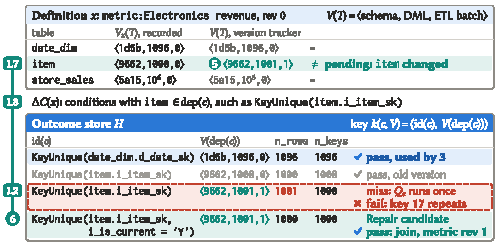
\includegraphics[width=\columnwidth]{figures/maintenance}%
\caption{\bt{Lookup after the \code{item} load (steps 5--6; L$n$ marks line $n$ of Algorithm~\ref{alg:maintenance}). Only \code{item}'s stamp changed, so only the \code{item} key check reruns, once, at its new key; the \code{date\_dim} outcome still serves three definitions.}{\code{item} 载入后的查找（步骤 5--6；L$n$ 指算法~\ref{alg:maintenance} 第 $n$ 行）。只有 \code{item} 的版本戳变化，因此只有 \code{item} 键检查在新键上重跑一次；\code{date\_dim} 的检查结果仍服务三个定义。}}
\label{fig:maintenance}
\Description{Top: the stamps of definition x, metric:Electronics revenue, revision 0, where a stamp V(T) is (schema fingerprint, DML count, ETL batch). For each table the recorded stamp V_x(T) is next to the version tracker's current stamp V(T): date_dim (1d5b, 1096, 0) equals (1d5b, 1096, 0); store_sales (5a15, 10^6, 0) equals itself; item (9662, 1000, 0) differs from (9662, 1001, 1), produced by the ETL load (step 5), so the definition is pending (tag L7). Tag L8: Delta C(x) is the set of conditions whose dep(c) contains item, such as KeyUnique(item.i_item_sk). Bottom: the outcome store H with key k(c, V) = (id(c), V(dep(c))) and columns n_rows and n_keys. Row 1, highlighted: KeyUnique(date_dim.d_date_sk) at (1d5b, 1096, 0), 1096 rows over 1096 keys, pass, used by 3. Row 2, grey: KeyUnique(item.i_item_sk) at (9662, 1000, 0), 1000 over 1000, pass, old version. Row 3, red dashed, tag L2: KeyUnique(item.i_item_sk) at (9662, 1001, 1), miss, Q_c runs once, 1001 rows over 1000 keys, fail: key 17 repeats. Row 4, step 6: KeyUnique(item.i_item_sk, i_is_current = 'Y') at (9662, 1001, 1), the Repair candidate, 1000 over 1000, pass, join and metric revision 1. A vertical line connects tags L7, L8, L2 and step 6 down the left edge.}
\end{figure}

\begin{algorithm}[t]
\caption{\bt{Two-stage validation and dual maintenance of $G$ and definitions}{两级验证及证据图 $G$ 与定义的双重维护}}
\label{alg:maintenance}
\small
\begin{algorithmic}[1]
\Require Revision $x$; state $D$; stamps $V$; batch $\Delta T$; stores $\mathcal H, G$
\Ensure Validated revision $x'$, pending diff, or $\bot$
\Function{EvalCond}{$c, D, V, \Delta T, \mathcal H$}
  \If{key $k(c, V)$ is not in $\mathcal H$}
    \State $\mathcal H[k(c, V)] \gets \operatorname{DeltaCheck}(c, \Delta T)$ if $\Delta T$ else $Q_c(D)$
  \EndIf
  \State \Return $\operatorname{Accept}(c, \mathcal H[k(c, V)])$
\EndFunction
\Function{ValidateAndMaintain}{$x, D, V, \Delta T, \mathcal H, G$}
  \IfThen{$V(\operatorname{dep}(x)) = V_x(\operatorname{dep}(x))$}{\Return $x$} \Comment{Stage 1 hit}
  \State $\Delta C(x) \gets \{c \in C(x) \mid V(\operatorname{dep}(c)) \neq V_x(\operatorname{dep}(c))\}$
  \For{each $c \in \Delta C(x)$ (base checks before rewrite premises)}
    \If{$\neg\Call{EvalCond}{c, D, V, \Delta T, \mathcal H}$}
      \For{each $(u, m, P) \in G$ with $c \in P$} \Comment{C2 revoke}
        \State Suspend $(u,m,P)$; revert $\Phi(m)$; roll back rewrite
      \EndFor
      \IfThen{$c$ is a probe check}{\Return $\text{Pending}(x, c, \Delta\text{vals})$}
      \State \Return $\operatorname{SingleEditRepair}(x, c, D, \mathcal H)$ \Comment{C3 repair}
    \EndIf
  \EndFor
  \State $V_x(\operatorname{dep}(x)) \gets V(\operatorname{dep}(x))$; \Return $x$
\EndFunction
\end{algorithmic}
\end{algorithm}

\bi{\emph{1. Two-stage write filtering and shared outcomes in $\mathcal H$.} Outside consumer transactions, a lightweight tracker maintains composite table stamps $V(T)$ (schema hash, DML counters, ETL batch ID) and flags insert-only batches $\Delta T$. The shared store $\mathcal H$ indexes condition outcomes by}
{\emph{1. 两级写入筛选与共享验证表 $\mathcal H$。}在消费端事务外，轻量跟踪器维护复合表版本戳 $V(T)$（模式哈希、DML 计数、ETL 批次号）并标记纯插入批次 $\Delta T$。共享结果表 $\mathcal H$ 按下式索引检查结果：}
\begin{equation}
\label{eq:condition-result-key}
k(c,V)=\bigl(\operatorname{id}(c),V(\operatorname{dep}(c))\bigr).
\end{equation}
\bi{After a write, \emph{Stage~1 (Table-stamp filter)} skips every condition whose dependency stamps $V(\operatorname{dep}(c))$ match $V_x$ (line 6 of Algorithm~\ref{alg:maintenance}), and shares each remaining check $\mathcal H[k(c,V)]$ across all definitions and agents referencing $\operatorname{id}(c)$ (in Figure~\ref{fig:maintenance}a, 3 definitions share one \code{date\_dim} check). \emph{Stage~2 (Insert-batch $\Delta T$ filter)} avoids full scans on insert-only batches $\Delta T$ (\textsc{EvalCond}, line 2): $\operatorname{KeyUnique}(T,K,\varphi)$ probes only $\sigma_\varphi(\Delta T) \bowtie T_{\mathrm{old}}$ via index lookups; dimension-join cardinality is skipped on fact appends; join completeness updates matched/unmatched counts incrementally from $\Delta T$; and $\operatorname{Dom}(T.a)\subseteq V_0$ inspects only $\Delta T.a$.}
{数据写入后，\emph{第一级（表版本筛选）}跳过依赖表版本未变的条件（算法~\ref{alg:maintenance} 第 6 行），并在引用同一签名 $\operatorname{id}(c)$ 的所有定义与智能体间共享 $\mathcal H[k(c,V)]$（图~\ref{fig:maintenance}a 中 3 个定义共享一次 \code{date\_dim} 检查）。对纯插入批次 $\Delta T$，\emph{第二级（插入批次增量筛选）}进一步避免全表扫描（\textsc{EvalCond} 第 2 行）：键唯一性仅经索引探查检验 $\sigma_\varphi(\Delta T) \bowtie T_{\mathrm{old}}$；事实追加跳过维表连接基数；连接完整性由 $\Delta T$ 增量更新计数；值域假设仅扫描 $\Delta T.a$。}

\bi{\emph{2. Dual maintenance of C2 premises and C3 definitions.} When a condition $c$ fails (lines 10--14 of Algorithm~\ref{alg:maintenance} and Figure~\ref{fig:maintenance}b), \system{} executes two branches:
\textbf{Branch 1 (C2 premise revocation):} Every certified equivalence edge $(u, m, P)$ in $G$ with $c\in P$ is suspended, grounded templates in $\Phi(m)$ routed via that edge revert to tentative, and any optimized revision derived from that rule rolls back to its parent.
\textbf{Branch 2 (C3 definition repair or suspension):} If $c$ is a probe-lifted domain condition ($\operatorname{Dom}(T.a)\subseteq V_0$), the data cannot decide whether new values $\Delta\text{vals}$ belong in the metric, so \system{} marks $m^r$ \emph{Pending} with $(c, \Delta\text{vals})$ for focused single-field inspection. If $c$ is a structural uniqueness or date-coverage check, \textsc{SingleEditRepair} tests exact-row deduplication, equality filters $T.col = v$ on low-cardinality columns ($\le 20$ values, e.g., \code{i\_is\_current = 'Y'}), or standard date-key encodings (\code{yyyymmdd} / day numbers), publishing $m^{r+1}$ \emph{iff} a \emph{unique} single edit restores all conditions in $C$ and reproduces the learning answer on the learning snapshot (and marking $m^r$ invalid $\bot$ otherwise).}
{\emph{2. C2 等价前提与 C3 定义的双重维护。}当条件 $c$ 失效时（算法~\ref{alg:maintenance} 第 10--14 行与图~\ref{fig:maintenance}b），系统执行两条分支：\textbf{分支 1（撤销 C2 等价前提）：}挂起图 $G$ 中所有满足 $c\in P$ 的认证等价边 $(u, m, P)$，将经由该边路由的接地模板退回待验证状态，并将该规则派生的优化版本回滚至父版本。\textbf{分支 2（修复或挂起 C3 定义）：}若 $c$ 为探针值域假设，数据无法判断新枚举值 $\Delta\text{vals}$ 是否归属该指标，系统将 $m^r$ 标为附带 $(c, \Delta\text{vals})$ 的 \emph{Pending} 状态以供定点复核；若 $c$ 为结构唯一性或日期覆盖条件，\textsc{SingleEditRepair} 搜索精确去重、低基数列（$\le 20$ 个取值，如 \code{i\_is\_current = 'Y'}）上的等值过滤或标准日期键重编码，\emph{当且仅当}存在\emph{唯一}单步补丁恢复全部条件 $C$ 并在学习快照上复现原核验答案时发布 $m^{r+1}$，否则标为失效（$\bot$）。}

\bi{\emph{3. Snapshot-bound execution ($\mathcal H_{\mathrm{tx}}$).} To prevent a concurrent write from committing between check and query execution, \code{CheckAndRun} (Figure~\ref{fig:maintenance}c) opens one read-only \code{REPEATABLE READ} transaction $s$. A statement-level trigger atomically increments a transactional counter $v(T)$ inside each write transaction, so any two snapshots reading identical counters $v_s(\operatorname{dep}(c))$ see identical table states. Inside $s$, \system{} reuses or evaluates $\mathcal H_{\mathrm{tx}}\bigl(\operatorname{id}(c), v_s(\operatorname{dep}(c))\bigr)$ and runs $q(D_s)$ in the exact same snapshot $s$.}
{\emph{3. 快照绑定执行（$\mathcal H_{\mathrm{tx}}$）。}为防止并发写入在检查与查询之间提交，\code{CheckAndRun}（图~\ref{fig:maintenance}c）开启单个只读 \code{REPEATABLE READ} 事务快照 $s$。语句级触发器在每次写入事务内原子递增计数器 $v(T)$，读到相同计数向量 $v_s(\operatorname{dep}(c))$ 的快照必看到完全相同的表状态。系统在快照 $s$ 内查验或计算 $\mathcal H_{\mathrm{tx}}\bigl(\operatorname{id}(c), v_s(\operatorname{dep}(c))\bigr)$，并在同一快照 $s$ 内执行编译查询 $q(D_s)$。}

\subsection{\bt{Shared Query Optimization and Rollback}{共享查询优化与回退}}
\label{sec:optimization}
\bi{The conditional rewrites R3 (date-key range selection under contiguity premise $P_{\mathrm{R3}}$) and R1 (redundant left-join removal under uniqueness premise $P_{\mathrm{R1}}$) from Proposition~\ref{prop:rewrite} also optimize published definitions. A candidate revision $m^{r+1}$ proposed via R3 or R1 is admitted in a repeatable-read snapshot iff: (1) any added premise ($P_{\mathrm{R3}}$) holds and enters $C(m^{r+1})$; (2) $m^{r+1}$ matches $m^r$ on the learning question, all 12 months of the learning year, a quarter, a period difference, and a monthly ranking; and (3) paired alternating executions across $\ge 8$ periods show a 95\% confidence interval for mean latency reduction entirely below zero with $\ge 10\%$ speedup. Because Algorithm~\ref{alg:maintenance} checks base conditions before rewrite premises (line 8), if a load breaks $P_{\mathrm{R3}}$, Branch~1 immediately suspends the R3 edge and rolls $m^{r+1}$ back to $m^r$.}
{命题~\ref{prop:rewrite} 的条件改写规则 R3（连续性前提 $P_{\mathrm{R3}}$ 下的日期键范围选择）与 R1（唯一性前提 $P_{\mathrm{R1}}$ 下的冗余左连接消除）同时用于优化已发布定义。候选版本 $m^{r+1}$ 在可重复读快照内须通过三项检验：（1）新增前提（$P_{\mathrm{R3}}$）成立并并入 $C(m^{r+1})$；（2）在学习题、学习年份 12 个月、季度、期间差值及月度排名上与 $m^r$ 结果一致；（3）至少 8 个期间的交替执行显示平均耗时降幅 $\ge 10\%$ 且配对均值差 95\% 置信区间完全小于 0。一旦后续写入破坏 $P_{\mathrm{R3}}$，算法~\ref{alg:maintenance} 分支 1 立即挂起 R3 边并将 $m^{r+1}$ 回滚至 $m^r$。}

\subsection{\bt{Predictive Feature Compilation and Reuse}{预测特征编译与跨任务复用}}
\label{sec:features}
\bi{Predictive tasks aggregate relative to per-instance entity keys and temporal cutoffs $(u_i,t_i)$~\cite{robinson2024relbench}. A feature revision $f^r$ extends $I$ with an entity mapping (target entity table/key, verified join path $\eta(x)$, optional anchor $a(u_i)$), look-back window $w$, and fill value. For a joined fact row $x\in J_I(D_s)$ with event time $t(x)$, compilation emits one PostgreSQL \code{LATERAL} subquery per feature aggregating rows where}
{预测任务围绕样本实体键与时间截点 $(u_i,t_i)$ 聚合~\cite{robinson2024relbench}。特征版本 $f^r$ 在 $I$ 上扩展实体映射（目标实体表与键、已验证连接路径 $\eta(x)$、可选锚属性 $a(u_i)$）、回看窗口 $w$ 与填充值。对连接后事实行 $x\in J_I(D_s)$ 及事件时间 $t(x)$，编译器为每条特征生成一条 PostgreSQL \code{LATERAL} 子查询，聚合满足下式的记录：}
\begin{equation}
\label{eq:feature-window}
\eta(x)=a(u_i),\qquad t_i-w<t(x)\leq t_i,
\end{equation}
\bi{excluding facts after $t_i$ to prevent temporal leakage. \system{} supports both complete \emph{task programs} for same-task retraining and modular \emph{feature definitions} composed across tasks sharing an entity (\code{find\_program}, \code{find\_features}, \code{compose\_features}). Candidate features from sessions beating the single-table baseline must pass four gates: valid fields and many-to-one joins, fact-grain uniqueness, exact column reproduction across 2,000 seeds, and identical outputs on time-censored views hiding rows after $t_i$. Published features share $\mathcal H$ and follow Algorithm~\ref{alg:maintenance} under updates.}
{严格排除 $t_i$ 之后的事实行以防时间泄漏。\system{} 同时支持用于同任务重训的\emph{任务程序}与跨任务组合的模块化\emph{特征定义}（\code{find\_program}、\code{find\_features}、\code{compose\_features}）。优于单表基线的候选特征须通过四项门禁：字段与多对一连接合法、事实粒度键唯一、在 2,000 个种子上逐值复现提交列，以及在隐去 $t_i$ 之后数据的截断视图上结果不变。发布特征共享 $\mathcal H$ 并按算法~\ref{alg:maintenance} 维护。}
